\section{Reflection in general}
\emph{Reflection} is the ability of a program to manipulate as data something representing the state of the program during its own execution.
A system may support reflection at different levels: from simple information on types to reflecting the entire structure of the program.
Another variant of reflection is if a program is allowed to only read or also to change itself.

\emph{Introspection} is the ability of a program to observe and therefore reason abut its own state.
\emph{Intercession} is the ability for a program to modify its own execution state or alter its own interpretation or meaning.
Both functionalities require a mechanism for encoding execution state as data.
Those mechanisms are called \emph{reification}.

\emph{Structural reflection} is the ability of the language to provide a complete reification of both the program currently executed and its abstract data types.

\emph{Behavioral reflection} is the ability of the language to provide a complete reification of its own semantics ad implementation, and the data and implementation of the run-time system.

\subsection{Uses of reflection}
Some of the main usage of reflection are:
\begin{itemize}
    \item class browsers: we use reflection in order to enumerate the members of classes;
    \item visual development environments: the know of the type information can help the developer in writing correct code;
    \item debuggers: can exploit reflections to examine private members of objects;
    \item test tools: can ensure high level of code coverage in a test suite;
    \item extensibility feature: an application may make use of external, user-defined classes by creating instances of extensibility objects.
\end{itemize}

\subsection{Drawbacks of reflection}
If it is possible to perform an action without the use of reflection, then it is preferable to avoid using it because:
\begin{itemize}
    \item reflection involves types that are dynamically resolved so optimizations cannot be performed so there is significant \emph{performance overhead};
    
    \item reflection requires a runtime permission which may not be present, so giving those permissions could lead to \emph{security problems};
    
    \item reflective code may access internals, so it can breaks abstractions and may change behaviour with upgrades of the platform, destroying portability.
\end{itemize}

\section{Reflection in Java}
Java supports introspection and reflexive invocation but not code modification.
For each data type (primitive, loaded or synthesized) the JVM maintains an associated object of class \verb|java.lang.Class| that reflects the type which represents.
That class is the entry point for reflection and all relevant information can be obtained from it.
The APIs are implemented inside the package \\ 
\verb|java.lang.reflect|.
\begin{figure}[H]
    \centering
    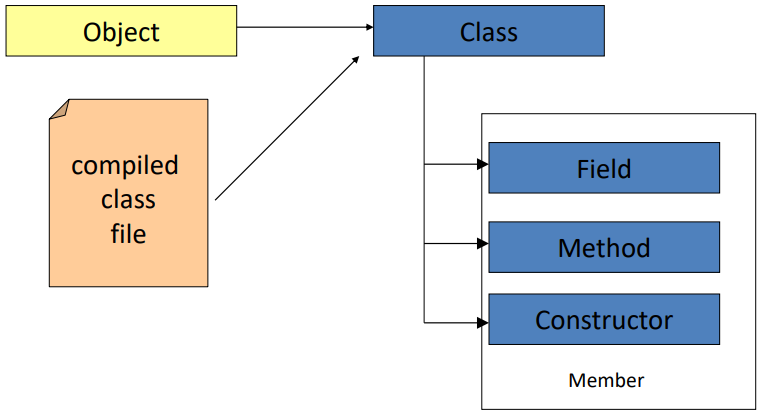
\includegraphics[width=350px]{images/4_Reflection/reflection_java.png}
    \caption{Reflection logical hierarchy in Java}
\end{figure}

\subsection{APIs}
First thing first to retrieve the Class object associated with the class we want to work with we use the method \verb|getClass| on an object of that type:
\begin{verbatim}
    Class c = "foo".getClass(); // get the Class object for the String type

    byte[] bytes = new byte[1024];
    Class c = bytes.getClass(); // get the Class object for the array type
    ...
\end{verbatim}
or we can use the property \verb|class| on the raw type (for primitive type too):
\begin{verbatim}
    Class c = String.class;
    Class c = boolean.class;
    Class c = int[][][].class;
\end{verbatim}
moreover we can get the instance by name using the method \verb|Class.forName(String)| in which we can specify the full path, or the jvm type name:
\begin{verbatim}
    Class c = Class.forName("java.util.List");
    Class c = Class.forName("[D");     // type name for double[]
    Class c = Class.forName("[[Ljava.lang.String"); // type name for String[][]
\end{verbatim}

Those instances represent classes and interfaces in a running Java application and are constructed automatically by the JVM as classes are loaded, basically providing access to the informations from the class file.

Some of the available APIs of the class objects are:
\begin{verbatim}
    // get the class name:
    String s = myClass.getName();
    
    // get the class modifiers:
    int m = myClass.getModifiers();
    Modifier.isPublic(m);
    Modifier.isAbstract(m);
    Modifier.isFinal(m);
    
    // check if is an interface:
    myClass.isInterface();
    
    // get the list of class objects who
    // represents the implemented interfaces
    Class[] itfs = myClass.getInterfaces();
    
    // get the superclass
    Class superclass = myClass.getSuperClass();
\end{verbatim}

Members of the class are modeled using some other classes similar to the \verb|Class| class, all inside the package \verb|java.lang.reflect.*| and all implementing the \verb|Member| interface.
Those objects can be retrieved using the following methods on the class object:
\begin{figure}[H]
    \centering
    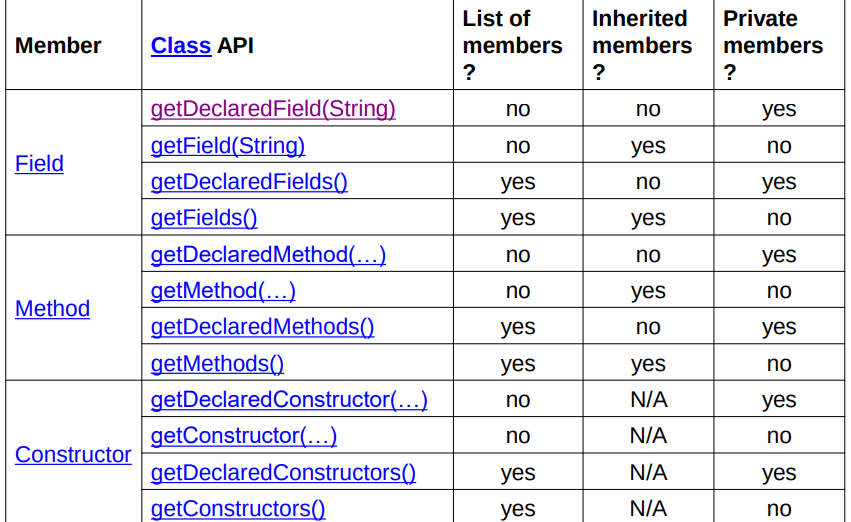
\includegraphics[width=400px]{images/4_Reflection/members_API.png}
    \caption{Methods for locating Members}
\end{figure}

So we have:
\begin{itemize}
    \item \verb|Member| interface;

    \item \verb|Field| class: have type and value as properties and the class provides methods for accessing type information and setting and getting values of a field on a given object;
    
    \item \verb|Method| class: have return type, parameters types and exception thrown as properties and the class provides methods for invoking the method on a given object;
    
    \item \verb|Constructor| class: have similar structure to the method one but constructor have no return values and the invocation of the constructor creates a new instance of an object instead of working on one already existing.
\end{itemize}

\subsubsection{Generic methods}
Due to Java's \emph{erasure semantics} generic type information is not represented at run time, so for example we have problems in using reflection over generics:
\begin{verbatim}
try{
    LinkedList<String> list = new LinkedList<String>();
    Class c = list.getClass();
    Method add = c.getMethod("add", String.class);
} catch(Exception e){
    System.out.println("Method not found");
}
\end{verbatim}
so executing the code above we will incurr in an exception because the method we are looking for cannot be found at runtime!
This version instead will work because type erasure will downgrade everything to Object:
\begin{verbatim}
try{
    LinkedList<String> list = new LinkedList<String>();
    Class c = list.getClass();
    Method add = c.getMethod("add", Object.class);
} catch(Exception e){
    System.out.println("Method not found");
}
\end{verbatim}

Moreover other than introspection we can use reflection to create new objects of a type that was not known at compile time and to access members that are not known at compile time.
For example to create an object using the default constructor we can:
\begin{verbatim}
Class c = Class.forName("java.awt.Rectangle");
Rectangle r = (Rectangle) c.newInstance();
\end{verbatim}
or using a constructor with some arguments:
\begin{verbatim}
// Get class we want to build from
Class c = Class.forName("java.awt.Rectangle");
// Create the array containing the types of parameters for the constructor
Class[] intArgsClass = new Class[]{int.class, int.class};
// Fetch the actual constructor
Constructor ctor = c.getConstructor(intArgsClass);

// Build the array of parameters for the constructor 
Object[] intArgs = new Object[]{new Integer(12), new Integer(24)};
// Call the constructor with the chosen parameters
Rectangle r = (Rectangle) ctor.newIstance(intArgs);
\end{verbatim}

In order to access the fields instead we can:
\begin{verbatim}
Rectangle r = new Rectangle(12, 24);

// Get the class
Class c = r.getClass();
// Get the field
Field f = c.getField("height");

// get property from the specified object: r.height
Integer h = (Integer) f.get(r);

// set property for the specified object: r.width=30;
f.set(r, new Integer(30));
\end{verbatim}

In order to invoke methods:
\begin{verbatim}
// Get class
Class c = String.class;
// Create array of parameter types classes
Class[] paramtypes = new Class[] {String.class};
// Get method concat for class String
Method concatMethod = c.getMethod("concat", paramtypes);

// Create array of actual parameters
Object[] args = new Object[] {s2};
// Call method with specified parameter
String result = (String) concatMethod.invoke(s1,args);
\end{verbatim}

\subsubsection{Forbidden actions}
Of course certain operations are forbidden by privacy rules:
\begin{itemize}
    \item changing final fields;
    \item reading or writing a private field;
    \item invoking a private method;
    \item ...
\end{itemize}
in case of that operation code will fail throwing the exception \verb|IllegalAccessException|.

There exists though a security manager that can allow or deny some of the actions above, so if the security managers allows them also those private fields can be accessed.

The \verb|AccessibleObject| is the super-class of all \verb|Field|, \verb|Method| and \verb|Constructor| and provides some useful methods:
\begin{itemize}
    \item \verb|isAccessible()|: gets the value of the accessible flag for that object;
    \item \verb|setAccessible(boolean)|: sets the accessibility flag for that object;
    \item \verb|static setAccessible(AccessibleObject[], boolean)|: sets the accessibility flag to the specified value to all the objects in the array.
\end{itemize}


\subsection{Example of usage in the JUnit framework}
Inside the JUnit framework we declare a class which contains tests, one method for each test and the method must start with the keyword \verb|test|, so in order to run those tests the basic mechanism of JUnit is.
\begin{verbatim}
public static void testDriver( String testClass ) {
    Class c = Class.forName( testClass );
    Object tc = c.newInstance( );
    Method[ ] methods = c.getDeclaredMethods( );
    for( int i = 0; i < methods.length; i++ ) {
    if( methods[ i ].getName( ).startsWith( "test" ) &&
        methods[ i ].getParameterTypes( ).length == 0 )
        methods[ i ].invoke( tc );
    }
}
\end{verbatim}


\section{Annotations}
Modifiers in Java (static, final, public) are meta-data describing properties of program elements, are reserved keyword so managed by the language.
Sometimes there is the need of additional meta-data to be specified by the programmer without of course changing the language itself.
We can think about annotations like a way for the user to define more of those modifiers.

\subsection{Structure of annotations}
Annotations are made of a \emph{name} and a finite number of \emph{attributes} pairs of the the kind \\
\verb|name = value|, but possibly none.
The syntaxes are:
\begin{itemize}
    \item \verb|@annName| for example \verb|@Override|;
    \item \verb|@annName{constExpression}| which is shorthand for specify value for single parameter annotations;
    \item \verb|@annName{name_1=constExp_1,...,name_k=constExp_k}|
\end{itemize}
it is to notice that as value can be only used const expression which are expression that can be computed at compile time!
Moreover the attributes have a type so the supplied values must be convertible to that type.

Annotations can be applied to almost any syntactic element:
\begin{itemize}
    \item package declarations;
    \item classes (enum variants too);
    \item interfaces (including annotations themselves);
    \item fields and local variables;
    \item methods and constructors;
    \item parameters;
    \item any type use.
\end{itemize}
can be used in any number with other modifiers.
Basically an annotation associates the name and set of specified attributes to the annotated element.

\subsection{Predefined annotations}
The java compiler itself defines and recognizes some predefined annotations, the user specified one are ignored on compilation but can be used by other tools (like javadoc, debuggers and more).
Some of the already predefined ones are:
\begin{itemize}
    \item \verb|@Override|: makes explicit the intention of the programmer that the declared method overrides a method defined in a superclass.
    Can be useful because during compilation the compiler specifies a warning if there is no method overridden;
    
    \item \verb|@Deprecated|: declares that the annotated elements not necessarily will be included in future releases of the Java API.
    During compilation the compiler will issue a warning to let the user know that the code is not future proof;
    
    \item \verb|@SuppressWarnings|: instructs the compiler to avoid issuing warnings for the specified situations (for example cast, deprecation, divzero, ecc, ecc).
    For example:
    \begin{verbatim}
        @SuppressWarnings({"deprecation" "empty"})
        void antiqueMethod(){
            OldClass.deprecateMethod();
        }
    \end{verbatim}

    \item \verb|@FunctionalInterface|: declares that an interface is functional (more on this in the functional part of Java).
\end{itemize}

\subsection{Define annotations}
Programmers can define new annotations to be used:
\begin{itemize}
    \item for documentation of the source;
    \item to implement tools that process the content of the \verb|.class| file;
    \item to inspect the annotations placed on a class at run-time.
\end{itemize}

The syntax to declare an annotation is the same as interface but starting with \verb|@interface|.
So basically an annotation type is an interface which defines fields which corresponds to the attributes we can specify in the annotation.
Example:
\begin{verbatim}
@interface InfoCode{
    String author ();
    String date ();
    int ver () default 1;
    int rev () default 0;
    String [] changes () default {};
}
\end{verbatim}
basically we have:
\begin{itemize}
    \item each method determines the name of an attribute and its type (specified by the return type);
    \item a default value can be specified for each attribute;
    \item attributes type can only be primitive type, String, Class, Enum, Annotation or an array of the specified types;
    \item additionally an annotation can contain constant declarations (with compile time initialization), internal classes and interfaces and enum.
\end{itemize}
Once the annotation has been declared can be applied to various program elements.

So for example:
\begin{verbatim}
@InfoCOde(author="Beppe", date="10/12/07")
public class C{
    public static void m1(){...}

    @InfoCode(author="Gianni", date="4/08/08",
            ver=1, rev=2)
    public static void m2(){...}
}
\end{verbatim}

\subsection{Annotate annotations}
Annotation definitions can be annotated to describe their meta-data.
Some of the predefined meta-annotations are:
\begin{itemize}
    \item \verb|@Target|: constrains the program elements to which the annotation can be applied.
    The value is an array of \verb|annotation.ElementType| which is an enum with the following variants:
    \begin{itemize}
        \item \verb|ANNOTATION_TYPE|
        \item \verb|CONSTRUCTOR|
        \item \verb|FIELD|
        \item \verb|LOCAL_VARIABLE|
        \item \verb|METHOD|
        \item \verb|PACKAGE|
        \item \verb|PARAMETER|
        \item \verb|TYPE_PARAMETER|
        \item \verb|TYPE_USE|
    \end{itemize}

    \item \verb|@Retention|: says until when the annotation should be present.
    The value is one of the variant of the enum \verb|annotation.RetentionPolicy| which are:
    \begin{itemize}
        \item \verb|SOURCE|
        \item \verb|CLASS|: which is the default
        \item \verb|RUNTIME|
    \end{itemize}
    
    \item \verb|@Inherited|: it's a marker annotation which is inherited by subclasses.
\end{itemize}

\subsubsection{Access annotations}
Annotations in class file can be used by appropriate tools for the program analysis and the package \verb|javax.annotations.processing| provides some useful APIs to help in developing such tools.

At run-time the annotations can be retrieved through reflection APIs for example:
\begin{itemize}
    \item \verb|Annotation[] getAnnotations()| in the Class object returns an array of \verb|Annotation| instances;
    \item \verb|<T extends Annotation> T getAnnotation(Class<T> annotationClass)| in the Method object returns the annotation of the specified type if it is present, otherwise it returns null.
\end{itemize}

NB: to access annotations of already loaded classes  we need to specify the retention policy to \verb|RUNTIME| otherwise that information will be discarded. 
